\documentclass[11pt]{article}
\usepackage[margin=1in]{geometry}
\usepackage{amsmath,amssymb,amsthm}
\usepackage{graphicx}
\usepackage{enumitem}
\usepackage{hyperref}
\usepackage{bm}

\newcommand{\Var}{\operatorname{Var}}
\newcommand{\Cov}{\operatorname{Cov}}
\newcommand{\E}{\mathbb{E}}
\newcommand{\tr}{\operatorname{tr}}
\newcommand{\R}{\mathbb{R}}
\newcommand{\Z}{\mathbb{Z}}
\newcommand{\N}{\mathbb{N}}

\title{Advanced Time Series Analysis PSET 1}
\author{Dhruv Kohli\thanks{Claude Code was used to assist with writing and debugging the Python code for Questions 3 and 4, and double checking my work and cleanliness of latex and presentation.}}
\date{Spring 2026}

\begin{document}
\maketitle

%% ====================================================================
\section{Question 1}
%% ====================================================================

\subsection{(i)}

We have that the $n\times n$ lag polynomial $C(L) = \sum_{\ell=0}^{\infty} C_\ell L^\ell$ satisfying the one-summability condition $\sum_{\ell=0}^{\infty} \ell |C_{ij,\ell}| < \infty$ for all $i,j$, and the lag polynomial $B(L) = \sum_{\ell=0}^{\infty} B_\ell L^\ell$ defined by
\[
B_\ell = -\sum_{m=\ell+1}^{\infty} C_m, \qquad \ell = 0,1,2,\ldots
\]
We want to show that $(I_n - L)\,B(L) = C(L) - C(1)$.

We compute $(I_n - L)\,B(L) = B(L) - L\,B(L)$ by collecting powers of $L$:
\begin{align*}
(I_n - L)\,B(L)
&= \sum_{\ell=0}^{\infty} B_\ell\, L^\ell \;-\; \sum_{\ell=0}^{\infty} B_\ell\, L^{\ell+1}
= \sum_{\ell=0}^{\infty} B_\ell\, L^\ell \;-\; \sum_{\ell=1}^{\infty} B_{\ell-1}\, L^{\ell} \\
&= B_0 + \sum_{\ell=1}^{\infty} \bigl(B_\ell - B_{\ell-1}\bigr)\, L^{\ell}.
\end{align*}

For $\ell \geq 1$, the coefficient differences are:
\[
B_\ell - B_{\ell-1}
= -\sum_{m=\ell+1}^{\infty} C_m - \Bigl(-\sum_{m=\ell}^{\infty} C_m\Bigr)
= \sum_{m=\ell}^{\infty} C_m - \sum_{m=\ell+1}^{\infty} C_m = C_\ell.
\]

For the constant term:
\[
B_0 = -\sum_{m=1}^{\infty} C_m
= C_0 - \sum_{m=0}^{\infty} C_m
= C_0 - C(1).
\]

Substituting back:
\[
(I_n - L)\,B(L) = C_0 - C(1) + \sum_{\ell=1}^{\infty} C_\ell\, L^\ell
= \sum_{\ell=0}^{\infty} C_\ell\, L^\ell - C(1)
= C(L) - C(1). \qedhere
\]

\subsection{(ii)}

We have $y_t = C(L)\,u_t$ with $u_t \sim \text{WN}(0,\Sigma)$ and $C(0)=I_n$. We want to show there exists a covariance stationary process $\{\eta_t\}$ such that $y_t = C(1)\,u_t + \eta_t - \eta_{t-1}$.
From part (i), we have $(I_n - L)\,B(L) = C(L) - C(1)$, i.e.,
\[
C(L) = C(1) + (1-L)\,B(L).
\]
Let $\eta_t \equiv B(L)\,u_t = \sum_{\ell=0}^{\infty} B_\ell\, u_{t-\ell}$. Since $B(L)$ is absolutely summable, $\eta_t$ is a well-defined, covariance stationary VMA$(\infty)$ process. Applying $C(L)$ to $u_t$ we get:
\[
y_t = C(L)\,u_t = C(1)\,u_t + (1-L)\,B(L)\,u_t = C(1)\,u_t + \eta_t - \eta_{t-1}.
\]

%% ====================================================================
\section{Question 2}
%% ====================================================================

We know $\{y_t\}$ and $\{x_t\}$ are scalar, jointly covariance stationary, mean-zero time series, with $y_t = C(L)\,u_t$, $C(0)=1$, $u_t \sim \text{WN}(0,\sigma_u^2)$, and $u_t \in \operatorname{sp}(y_\tau,\, -\infty < \tau \le t)$. Since $y_t = C(L)\,u_t$ implies $\operatorname{sp}(y_\tau,\,\tau\le t) \subseteq \operatorname{sp}(u_\tau,\,\tau\le t)$, and $u_t \in \operatorname{sp}(y_\tau,\,\tau\le t)$ gives the reverse inclusion, we have
\[
\operatorname{sp}(y_\tau,\,-\infty<\tau\le t) = \operatorname{sp}(u_\tau,\,-\infty<\tau\le t).
\]

\subsection{(i)}

We want to show that $\Var^*(y_{t+1} \mid \{y_\tau\}_{-\infty<\tau\le t}) = \sigma_u^2$.

By the span equality above, $(y_\tau,\,\tau\le t) = (u_\tau,\,\tau\le t)$. We then get:
\[
y_{t+1} = \sum_{\ell=0}^{\infty} C_\ell\, u_{t+1-\ell} = C_0\, u_{t+1} + \sum_{\ell=1}^{\infty} C_\ell\, u_{t+1-\ell}.
\]
The second sum lies in $(u_\tau,\,\tau \le t)$, and since $u_t$ is white noise, $E^*(u_{t+1} \mid \{u_\tau\}_{\tau\le t}) = 0$. Therefore:
\[
E^*(y_{t+1} \mid \{y_\tau\}_{\tau \le t}) = \sum_{\ell=1}^{\infty} C_\ell\, u_{t+1-\ell}.
\]
The forecast error is $y_{t+1} - E^*(y_{t+1} \mid \{y_\tau\}_{\tau\le t}) = C_0\, u_{t+1} = u_{t+1}$ (since $C_0=1$), so
\[
\Var^*(y_{t+1} \mid \{y_\tau\}_{\tau \le t}) = \E[u_{t+1}^2] = \sigma_u^2.
\]

\subsection{(ii)}

We want to show that $\Var^*(y_{t+1} \mid \{y_\tau,x_\tau\}_{\tau\le t}) = \Var^*(u_{t+1} \mid \{u_\tau,x_\tau\}_{\tau\le t})$.

By the span equality, $(y_\tau,\,\tau\le t) = (u_\tau,\,\tau\le t)$, so $(y_\tau,x_\tau;\,\tau\le t) = (u_\tau,x_\tau;\,\tau\le t)$.

Then
\[
y_{t+1} = u_{t+1} + \sum_{\ell=1}^{\infty} C_\ell\, u_{t+1-\ell},
\]
where $\sum_{\ell=1}^{\infty} C_\ell\, u_{t+1-\ell} \in (u_\tau,\,\tau\le t) \subseteq (u_\tau,x_\tau;\,\tau\le t)$. Therefore:
\[
E^*\bigl(y_{t+1} \mid \{u_\tau,x_\tau\}_{\tau\le t}\bigr) = E^*\bigl(u_{t+1} \mid \{u_\tau,x_\tau\}_{\tau\le t}\bigr) + \sum_{\ell=1}^{\infty} C_\ell\, u_{t+1-\ell},
\]
so the forecast error is:
\[
y_{t+1} - E^*(y_{t+1} \mid \cdots) = u_{t+1} - E^*(u_{t+1} \mid \{u_\tau,x_\tau\}_{\tau\le t}).
\]
Taking the variance of both sides and using $(y_\tau,x_\tau;\,\tau\le t) = (u_\tau,x_\tau;\,\tau\le t)$ gives
$\Var^*(y_{t+1} \mid \{y_\tau,x_\tau\}_{\tau\le t}) = \Var^*(u_{t+1} \mid \{u_\tau,x_\tau\}_{\tau\le t})$.

\subsection{(iii)}

We want to show that $\sigma_u^2 = \Var^*(u_{t+1} \mid \{u_\tau,x_\tau\}_{\tau\le t})$ if and only if $\Cov(u_{t+1},x_{t-\ell})=0$ for all $\ell\ge 0$.

Since $u_t \sim \text{WN}(0,\sigma_u^2)$, we have $u_{t+1} \perp (u_\tau,\,\tau\le t)$ (orthogonal in $L^2$). Therefore:
\[
E^*(u_{t+1} \mid \{u_\tau,x_\tau\}_{\tau\le t}) = 0 \quad\Longleftrightarrow\quad u_{t+1} \perp (u_\tau,x_\tau;\,\tau\le t).
\]
Since $u_{t+1}$ is already orthogonal to all $u_\tau$ ($\tau\le t$), the orthogonality to the entire joint span holds if and only if $u_{t+1} \perp x_{t-\ell}$ for all $\ell \ge 0$, i.e., $\Cov(u_{t+1},x_{t-\ell})=0$ for all $\ell \ge 0$.

When this holds, $E^*(u_{t+1} \mid \cdots) = 0$ and $\Var^*(u_{t+1}\mid\cdots) = \E[u_{t+1}^2] = \sigma_u^2$. Conversely, if $\Var^* = \sigma_u^2$, then the projection equals zero (since $\Var^* = \sigma_u^2 - \E[(E^*(\cdots))^2]$), which implies the orthogonality conditions.

\subsection{(iv)}

We want to show that for any $\ell \in \Z \cup \{\infty\}$,
\[
E^*\bigl(x_t \mid \{y_\tau\}_{-\infty<\tau\le t+\ell}\bigr) = \sum_{m=-\infty}^{\ell} a_m\, u_{t+m}, \qquad a_m = \frac{\Cov(x_t,\,u_{t+m})}{\sigma_u^2}.
\]

By the span equality, $(y_\tau,\,\tau\le t+\ell) = (u_\tau,\,\tau\le t+\ell)$. The best linear predictor of $x_t$ given $\{u_\tau\}_{\tau\le t+\ell}$ is a linear combination $\hat{x}_t = \sum_{m=-\infty}^{\ell} a_m\,u_{t+m}$.

By orthogonality, the coefficients $a_m$ must satisfy:
\[
\E\bigl[(x_t - \hat{x}_t)\,u_{t+k}\bigr] = 0 \quad \text{for all } k \le \ell.
\]
Which gives:
\[
\E[x_t\,u_{t+k}] - \sum_{m=-\infty}^{\ell} a_m\, \E[u_{t+m}\,u_{t+k}] = 0.
\]
Since $u$ is white noise, $\E[u_{t+m}\,u_{t+k}] = \sigma_u^2\,\mathbf{1}(m=k)$. Thus we conclude that:
\[
\Cov(x_t,\,u_{t+k}) - a_k\,\sigma_u^2 = 0 \quad \Longrightarrow \quad a_k = \frac{\Cov(x_t,\,u_{t+k})}{\sigma_u^2}.
\]

\subsection{(v)}

We want to show that:
\[
\Var^*(y_{t+1} \mid \{y_\tau,x_\tau\}_{\tau\le t}) = \Var^*(y_{t+1} \mid \{y_\tau\}_{\tau\le t})
\]
if and only if
\[
\Var^*(x_t \mid \{y_\tau\}_{-\infty<\tau<\infty}) = \Var^*(x_t \mid \{y_\tau\}_{\tau\le t}).
\]

By (i) and (ii):
\[
\text{LHS} \;\Longleftrightarrow\; \Var^*(u_{t+1} \mid \{u_\tau,x_\tau\}_{\tau\le t}) = \sigma_u^2.
\]
By (iii), this holds if and only if $\Cov(u_{t+1}, x_{t-\ell}) = 0$ for all $\ell \ge 0$. By stationarity, this is equivalent to
\begin{equation}\label{eq:cond}
a_m = \frac{\Cov(x_t, u_{t+m})}{\sigma_u^2} = 0 \quad \text{for all } m \ge 1.
\end{equation}

By (iv) with $\ell = 0$:
\[
E^*(x_t \mid \{y_\tau\}_{\tau\le t}) = \sum_{m=-\infty}^{0} a_m\, u_{t+m}.
\]
By (iv) with $\ell = \infty$:
\[
E^*(x_t \mid \{y_\tau\}_{-\infty<\tau<\infty}) = \sum_{m=-\infty}^{\infty} a_m\, u_{t+m}.
\]
Therefore:
\begin{align*}
\Var^*(x_t \mid \{y_\tau\}_{\tau\le t}) - \Var^*(x_t \mid \{y_\tau\}_{-\infty<\tau<\infty})
&= \E\bigl[(E^*(x_t \mid \text{all}))^2\bigr] - \E\bigl[(E^*(x_t \mid \text{past}))^2\bigr] \\
&= \sum_{m=1}^{\infty} a_m^2\,\sigma_u^2.
\end{align*}
So $\Var^*(x_t \mid \{y_\tau\}_{-\infty<\tau<\infty}) = \Var^*(x_t \mid \{y_\tau\}_{\tau\le t})$ if and only if $a_m = 0$ for all $m \ge 1$.

Both sides reduce to the same condition ($a_m = 0$ for all $m \ge 1$) which completes the proof.

%% ====================================================================
\section{Question 3}
%% ====================================================================

\subsection{(i)}

We transform the Federal Funds Rate to quarterly averages. Real GDP and the GDP deflator are transformed to annualized quarter-over-quarter log growth rates: $400 \times \Delta\log(X_t)$.

The three VAR variables are:
\begin{enumerate}
\item Real GDP growth: $y_{1,t} = 400\,\Delta\log(\text{GDPC1}_t)$,
\item GDP deflator inflation: $y_{2,t} = 400\,\Delta\log(\text{GDPDEF}_t)$,
\item Real rate spread: $y_{3,t} = \text{FEDFUNDS}_t - y_{2,t}$.
\end{enumerate}

We fix the effective sample size across all lag orders by setting aside the first $p_{\max} = 20$ observations as the conditioning set. This gives a fixed effective sample of $T = 242$ for every $p$. We compute the BIC and AIC, which give:
\begin{center}
BIC selects $p = 1$. \qquad AIC selects $p = 11$.
\end{center}

\begin{figure}[h!]
\centering
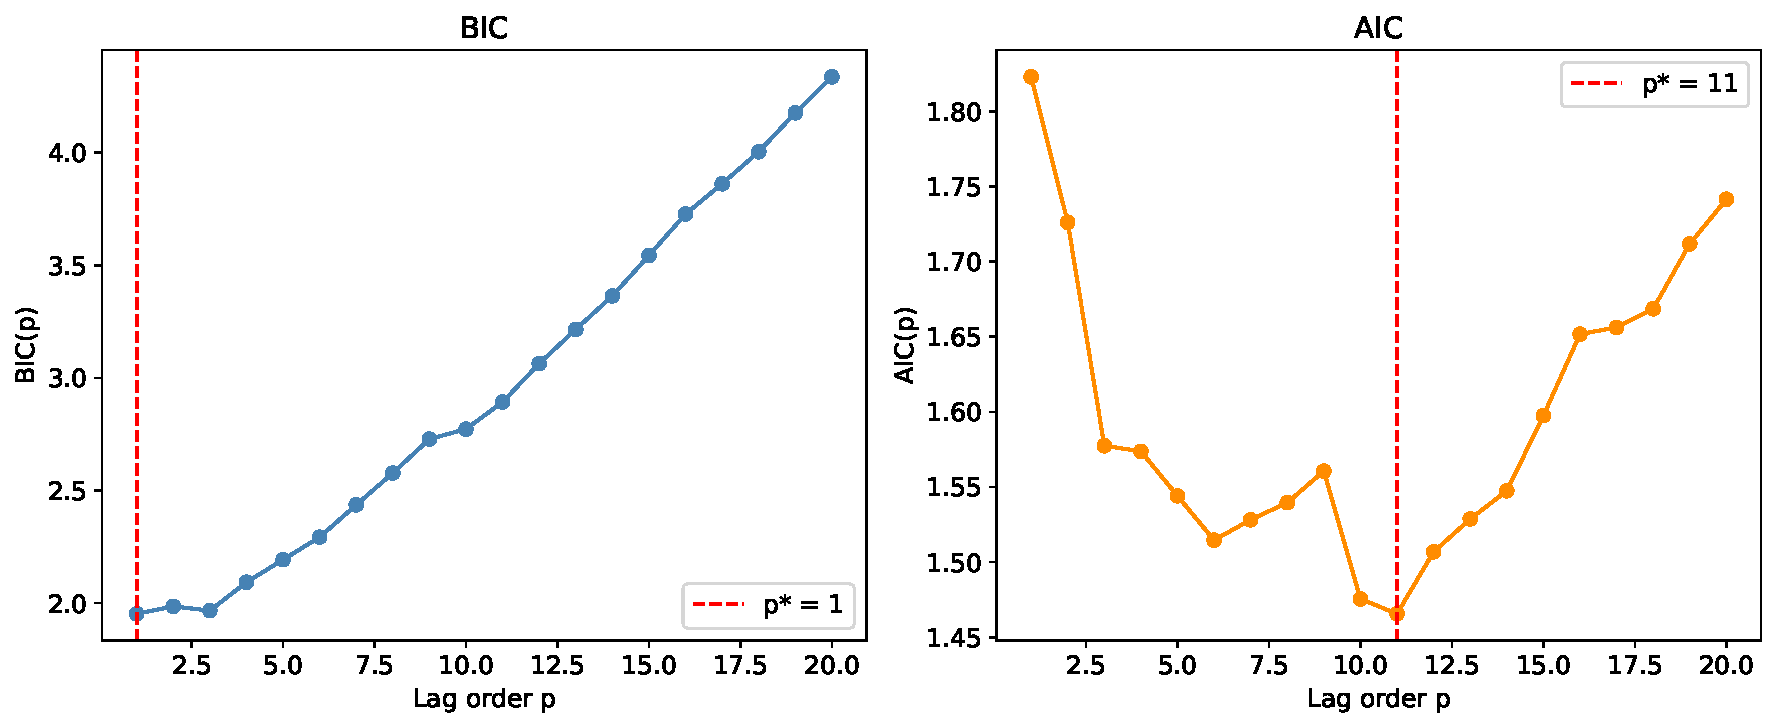
\includegraphics[width=0.75\textwidth]{q3_bic_aic.pdf}
\caption{BIC and AIC as functions of VAR lag order $p$.}
\end{figure}

%% ====================================================================
\section{Question 4}
%% ====================================================================

We use a conjugate NIW prior:
\[
\Sigma \sim \text{IW}(\Psi, d), \qquad (\beta \mid \Sigma) \sim N(b, \Sigma \otimes \Omega),
\]
with $d = n+2 = 5$, $\Psi = (d-n-1)\cdot 0.02^2\, I_n = 0.0004\, I_3$, $b = 0$. We now derive the diagonal matrix $\Omega$.

We know that $\Var(C \mid \Sigma) = 10^2\,\Sigma$, which gives $\Omega_{1,1} = 100$. For the lag coefficients:
\[
\Cov(B_{ij,s},\,B_{hm,r} \mid \Sigma)
= \frac{0.2^2}{0.02^2/(d-n-1)}\;\frac{1}{s^2}\;\Sigma_{ih}
= \frac{100}{s^2}\;\Sigma_{ih},
\qquad m = j,\; r = s.
\]
In the Kronecker structure $\Cov(\beta \mid \Sigma) = \Sigma \otimes \Omega$, the element
$\Cov(B_{ij,s},\,B_{hm,r}\mid\Sigma) = \Sigma_{ih}\cdot\Omega_{(s-1)n+1+j,\,(r-1)n+1+m}$,
so we need
\[
\Omega_{(s-1)n+1+j,\,(s-1)n+1+j} = \frac{100}{s^2}, \qquad s=1,\ldots,p,\; j=1,\ldots,n.
\]

\subsection{(i)}

We condition on the first $p_{\max}=20$ observations and use the resulting fixed effective sample $T = T_{\text{full}} - p_{\max} = 242$ for all lag orders, so that the marginal likelihoods are directly comparable. We compute the log marginal likelihood for each $p = 0,1,\ldots,20$ using the expression in the GLP notes:
\begin{align*}
\log p(Y \mid \gamma) &= -\frac{nT}{2}\log(\pi) + \log\Gamma_n\!\Bigl(\frac{T+d}{2}\Bigr) - \log\Gamma_n\!\Bigl(\frac{d}{2}\Bigr)
- \frac{T}{2}\log|\Psi| \\
&\quad - \frac{n}{2}\log\bigl|D_{\Omega}'\,x'x\,D_{\Omega} + I_k\bigr|
- \frac{T+d}{2}\log\bigl|I_n + D_{\Psi}'\,S\,D_{\Psi}\bigr|,
\end{align*}
where $T$ denotes the effective sample size, $D_\Omega D_\Omega' = \Omega$, $D_\Psi D_\Psi' = \Psi^{-1}$, $\hat{B} = (x'x + \Omega^{-1})^{-1}x'y$, and $S = \hat{\varepsilon}'\hat{\varepsilon} + \hat{B}'\Omega^{-1}\hat{B}$.

\begin{figure}[h!]
\centering
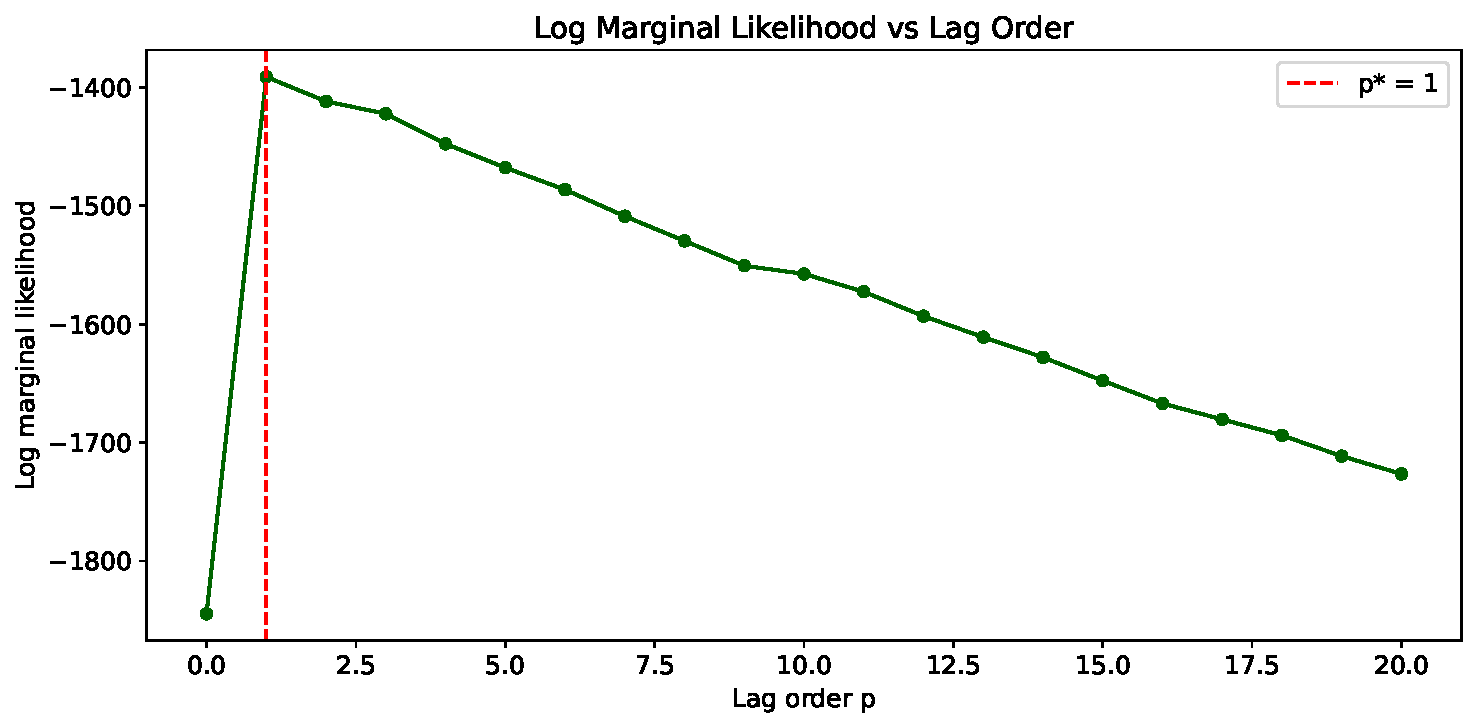
\includegraphics[width=0.75\textwidth]{q4i_logml.pdf}
\caption{Log marginal likelihood as a function of the VAR lag order $p$.}
\label{fig:q4i}
\end{figure}

The log marginal likelihood peaks at $p^* = 1$ (Figure~\ref{fig:q4i}) and decreases for $p > 1$, so we have a clear optimal $p^* = 1$ to choose.

\subsection{(ii)}

Using $p^* = 1$, we draw from the posterior predictive distribution of real GDP growth in 2020-Q2. We do so using the following steps:

\begin{enumerate}
\item Draw $\Sigma^{(i)}$ from the posterior $\text{IW}\!\bigl(\Psi + S,\; T+d\bigr)$.
\item Draw $B^{(i)} \mid \Sigma^{(i)}$ from $N\!\bigl(\text{vec}(\hat{B}),\;\Sigma^{(i)} \otimes (x'x + \Omega^{-1})^{-1}\bigr)$.
\item Given $(B^{(i)}, \Sigma^{(i)})$ and the observed data, simulate $y_{T+1}^{(i)}$ and then $y_{T+2}^{(i)}$ from the VAR model.
\item Record $y_{1,T+2}^{(i)}$, the real GDP growth component.
\item Repeat steps 1--4 for $i = 1,\ldots,20{,}000$ to approximate the marginal predictive density.
\end{enumerate}

\begin{figure}[h!]
\centering
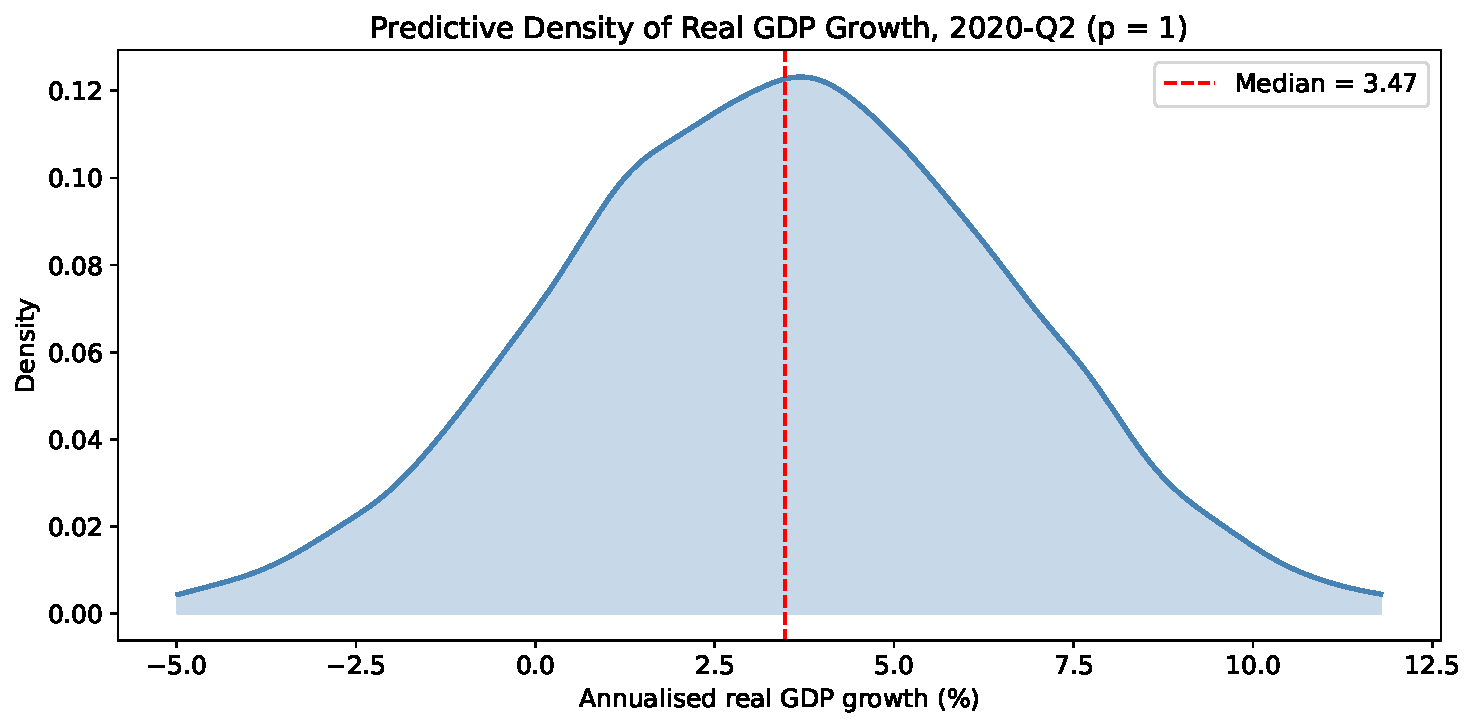
\includegraphics[width=0.75\textwidth]{q4ii_pred_density.pdf}
\caption{Posterior predictive density of annualized real GDP growth in 2020-Q2.}
\end{figure}

The posterior predictive distribution is approximately normal, centered around $3.4\%$ annualized growth, with a standard deviation of about $3.2$ percentage points. The 90\% credible interval is roughly $[-1.9\%,\; 8.6\%]$ which is pretty far off from the actual due to the COVID shock. 

\end{document}
